%-*- tex; tabsize:2; -*- %%%%%%%%%%%%%%%%%%%%%%%%%%%%%%%%%%%%%%%%%%%%%%%%%%%
%
%                          Copyright 2004 JASSPA.
%                           All Rights Reserved
%
%
%  System        : MicroEmacs
%  Module        : user Manual
%  Object Name   : $RCSfile: jasspame.tex,v $
%  Revision      : $Revision: 1.1 $
%  Date          : $Date: 2005-03-10 01:00:55 $
%  Author        : $Author: jon $
%  Created By    : Jon Green
%  Created       : Mon Oct 25 21:36:13 2004
%  Last Modified : <050310.0049>
%
%  Description
%
%  Notes
%
%  History
%
%  $Log: not supported by cvs2svn $
%
%%%%%%%%%%%%%%%%%%%%%%%%%%%%%%%%%%%%%%%%%%%%%%%%%%%%%%%%%%%%%%%%%%%%%%%%%%%%%
%
% Copyright (c) 2004 JASSPA.
%
% All Rights Reserved.
%
% This  document  may  not, in  whole  or in  part, be  copied,  photocopied,
% reproduced,  translated,  or  reduced to any  electronic  medium or machine
% readable form without prior written consent from JASSPA.
%
%%%%%%%%%%%%%%%%%%%%%%%%%%%%%%%%%%%%%%%%%%%%%%%%%%%%%%%%%%%%%%%%%%%%%%%%%%%%%

\documentclass[11pt,a4paper,pdftex]{article}
% Bring in the CVS information.
\def\CVS$#1: #2 ${\expandafter\def\csname CVS#1\endcsname{#2}}
\CVS$Revision: 1.1 $ % or any CVS keyword
\CVS$Date: 2005-03-10 01:00:55 $

\usepackage{ifthen}                     % Conditional processing.

\newboolean{Colorlinks}
\setboolean{Colorlinks}{true}              % For colored links

% Document information
%\newcommand{\docAuthor}{Jon Green, Kevin Garvey}
\newcommand{\docAuthor}{Jon Green}
\newcommand{\docSubject}{JASSPA MicroEmacs}
\newcommand{\docTitle}{Getting Started with JASSPA MicroEmacs}
\newcommand{\docDate}{\CVSDate}
\newcommand{\docVersion}{\CVSRevision}
\newcommand{\docReference}{jasspame}

% Import the font packages.
%\usepackage[latin1]{inputenc}          % We do not seem to need this
\usepackage{eurosym}                    % Use the Euro symbol for "\euro"
\usepackage[T1]{fontenc}                % Refer to TeX psnfss2e.pdf
\usepackage{textcomp}                   % Refer to TeX psnfss2e.pdf
\usepackage{aecompl}                    % AE complement to T1 for "\NG" and "\ng"
%
% FONTS: The document is typeset in the following fonts:-
% roman:      Times-Roman
% sans serif: Helvetica (scaled at .92)
% typewriter: Courier
\usepackage{courier}
\usepackage[scaled=0.92]{helvet}
%\usepackage{utopia}
\renewcommand{\rmdefault}{ptm}  % Roman font is Times-Roman
%\renewcommand{\rmdefault}{put}  % Utopia font is Times-Roman
\renewcommand{\sfdefault}{phv}  % Sans serif font is helvetica
\renewcommand{\ttdefault}{pcr}  % Typewriter font is courier

% Change the default font to Helvetica.
%\usepackage{bookman}
%\renewcommand{\familydefault}{\sfdefault}
%\renewcommand{\sfdefault}{ppl}

% Import the font packages.
\usepackage{pslatex}
\usepackage{longtable}                  % Long split table environment.
\usepackage{graphicx}                   % Picture import package
\usepackage{fancyhdr}                   % Use fancy headers
\usepackage[numbers]{natbib}            % Use Natural Sciences Citations and References

% Detect, if we are using pdftex to create pdf output. The following
% code should better be in a LaTeX package...
\makeatletter
\newif\ifpdfoutput
\@ifundefined{pdfoutput}%
  {\let\pdfoutput\@undefined}%
  {\ifcase\pdfoutput
     \let\pdfoutput\@undefined
   \else
     \pdfoutputtrue
   \fi
  }%
\makeatother

\usepackage{geometry,mflogo,xspace,path,bm}
\newcommand{\psext}{ps}
\newcommand{\pdfext}{pdf}
\newcommand{\dviext}{dvi}

% Set up the default link colour
\ifthenelse{\boolean{Colorlinks}}
{%
  \newcommand{\Linkcolor}{blue}
  \newcommand{\Citecolor}{red}
  \newcommand{\Urlcolor}{blue}
}
{%
  \newcommand{\Linkcolor}{black}
  \newcommand{\Citecolor}{black}
  \newcommand{\Urlcolor}{black}
}

\ifpdfoutput
  \pdfcompresslevel9
  \usepackage[colorlinks,bookmarks]{hyperref}
  \hypersetup{
    pdfauthor={\docAuthor},
    pdftitle={\docTitle},
    pdfsubject={\docSubject},
    pdfcreator={SunOS 5.9(sparc) - e-TeX(Web2C 7.5.2)},
    pdfkeywords={Emacs,MicroEmacs,Me,JASSPA},
    linkcolor={\Linkcolor},
    citecolor={\Citecolor},
    urlcolor={\Urlcolor},
    bookmarksnumbered=true,
    bookmarksopen=true
  }
  \usepackage{thumbpdf}
  \let\docext=\pdfext
\else
  \let\docext=\dviext
  \usepackage[bookmarks]{hyperref}
\fi

\title{\docTitle}
\author{Jon Green}
\date{\docDate}
%
% Bottom of the pages are ragged.
\raggedbottom
%
% Change the page width
%
\setlength{\marginparsep}{0pt}
\setlength{\marginparwidth}{0pt}
\addtolength{\textwidth}{.75in}
\addtolength{\hoffset}{-.25in}

\pagestyle{fancy}
% Set up the page.
% There is 1 inch at the top, reduce this to 0.4 inch.
\addtolength{\voffset}{-.6in}
\addtolength{\textheight}{.6in}
% We are adding a 1/2 inch graphic adjust the page sizes.
\setlength{\headheight}{.5in}
% Push page length to the bottom.
\addtolength{\textheight}{.5in}

%% Save the header image in a box
\newsavebox\HeaderImage
\savebox\HeaderImage{
\includegraphics[keepaspectratio,height=0.5in]{logo}}
% Redefine the header and footer for an alternative style.
\renewcommand{\sectionmark}[1]{\markright{\thesection\ #1}}
\fancyhf{}          % Delete the current header and footer
\fancyhead[EL,OR]{\bfseries\docTitle \\ \bfseries\rightmark}
\fancyhead[LO,RE]{\usebox{\HeaderImage}}
\fancyfoot[OL,ER]{{\small{Copyright {\textcopyright} 2004 JASSPA.}}\linebreak
                   \textit{\small{\docReference~~v\docVersion~~\docDate}}}
\fancyfoot[EL,OR]{\textsf{\large \textbf{\thepage}}}
\renewcommand{\headrulewidth}{1.5pt}%
\renewcommand{\footrulewidth}{1.5pt}%

% Redefine a plain header and footer than is absent for the
% front page.
\fancypagestyle{plain}{%
  % Watermark for the first header. First we clear down the
  % existing header that may be defined.
  \fancyhead{}%
  % Refer to the "Using Imported Graphics in LaTeX2"
  % Define the header to appear on the left hand edge of the page.
  % The picture dimensions are specified as (0,0), this means that
  % it occupies zero space (as far as the layout engine is concerned).
  % Appearing in the header means that they are rendered before the
  % page itself.
  % The image is placed 0 inches to the left and -10inches below
  % the header. The graphics are then included such that the
  % aspect ratio is maintained and the image width is as wide as
  % the text width.
  \fancyhead[OL,ER]{\setlength{\unitlength}{1in}
%             \begin{picture}(0,0)
%               \put(0,-10){\includegraphics[keepaspectratio,width=\textwidth]{watermark}}
%             \end{picture}
  }
  \renewcommand{\headrulewidth}{0pt}  % Remove line
  \fancyfoot[EL,OR]{}
}

\newcommand{\tableTitle}[1]{\textbf{#1}}%   % used on all table titles.

\begin{document}
\pagenumbering{roman}           %%% Roman page numbers for ToC

%%%%%%%%%%%%%%%%%%%%%%%%%%%%%%%%%%%%%%%%%%%%%%%%%%%%%%%%%%%%%%%%%%%%%%%%%%%%%%
%  Title Page                                                                %
%%%%%%%%%%%%%%%%%%%%%%%%%%%%%%%%%%%%%%%%%%%%%%%%%%%%%%%%%%%%%%%%%%%%%%%%%%%%%%
\thispagestyle{plain}
% The top header is the document information and the company logo. This is
% made up of 2 parbox's to get the correct horizontal wrapping that is
% required.
\parbox{2in}{
\includegraphics[keepaspectratio,width=1.9in]{logo}}
\hfill
\parbox{3.25in}{\sloppy
                \hfill\textsf{\huge JASSPA}
                \begin{flushright}
                  \textsf{\textbf{\Huge \docTitle}}
                \end{flushright}
                \hfill\textsf{\huge Version \docVersion}

                \hfill\textsf{\docAuthor}}
% The text information at the bottom of the page containing a copyright notice
% and contact details. This placed in a table and then shunted to the bottom
% of the page.
\begin{table}[b]
  \begin{center}
    \begin{tabular}{p{3in}p{3in}}
      \textsf{JASSPA}\vspace{6pt} & \\
      \textsf{\href{http://www.jasspa.com}{www.jasspa.com}\newline
              \href{mailto:support@jasspa.com}{support@jasspa.com}} & \\
%      \textsf{\sloppy\textbf{Copyright Notification:} No part of this
%      publication may be reproduced except as authorised by written
%      permission. The copyright and the foregoing restriction extend to
%      reproduction in all media.}
    \end{tabular}
  \end{center}
\end{table}

%%%%%%%%%%%%%%%%%%%%%%%%%%%%%%%%%%%%%%%%%%%%%%%%%%%%%%%%%%%%%%%%%%%%%%%%%%%%%%
%  Revision History                                                          %
%%%%%%%%%%%%%%%%%%%%%%%%%%%%%%%%%%%%%%%%%%%%%%%%%%%%%%%%%%%%%%%%%%%%%%%%%%%%%%
\newpage
% Change the format of the document to European paragraph spacing.
\setlength{\parindent}{0pt}
%\setlength{\parskip}{1ex plus 0.5ex minus 0.2ex}
\setlength{\parskip}{0.5ex}
\pagestyle{fancy}

\begin{small}
\vspace{.5in}
JASSPA.
\href{http://www.jasspa.com}{www.jasspa.com}\newline
\href{mailto:support@jasspa.com}{support@jasspa.com}\newline

\vspace{0.5in}

\textit{Copyright \textcopyright\ 2004 JASSPA.}

% \textit{Copyright}

\vspace{0.5in}

\begin{table}[ht]
  \begin{tabular}{ll}
    Title:        & \docTitle \\
    Reference:    & \docReference \\
    Version       & v\docVersion \\
    Date:         & \docDate \\
  \end{tabular}
\end{table}

Typeset with the TexLive 2003 \LaTeX\ Documentation System under Sun Solaris 9.

\vspace{0.5in}

\begin{center}
  \begin{table}[ht]
    \begin{tabular}{|c|c|p{4in}|c|}
    \hline
    \tableTitle{Date} & \tableTitle{Who} & \tableTitle{Description} & \tableTitle{Revision} \\
    \hline
    2004/10/25 & Jon & Draft. & 1.00 \\ \hline
    \end{tabular}
  \end{table}
\end{center}
\end{small}

%%%%%%%%%%%%%%%%%%%%%%%%%%%%%%%%%%%%%%%%%%%%%%%%%%%%%%%%%%%%%%%%%%%%%%%%%%%%%%
% Introduction                                                               %
%%%%%%%%%%%%%%%%%%%%%%%%%%%%%%%%%%%%%%%%%%%%%%%%%%%%%%%%%%%%%%%%%%%%%%%%%%%%%%
\newpage
% Change the format of the document to European paragraph spacing.
\setlength{\parindent}{0pt}
%\setlength{\parskip}{1ex plus 0.5ex minus 0.2ex}
\setlength{\parskip}{0.5ex}
\pagestyle{fancy}

%\textbf{\Large Preface}
\pdfbookmark[1]{Preface}{intro}    %%% additional bookmark for ref
\markboth{Preface}{Preface}   %%% for the page header
\section*{Preface}
%\addcontentsline{toc}{section}{\numberline{}Preface}

Time is short, and armed with a reasonable \LaTeX\ boiler plate it is time to
put down some usable notes on getting up and running with JASSPA MicroEmacs.
The on-line help that comes with JASSPA MicroEmacs details every public
function and variable in the editor however it is not that accessible and
certainly does not help the new user.

In this first draft, that will undoubtedly grow over time, we simply present
the post installation configuration to help the new user get up and running
with the editor.

%%%%%%%%%%%%%%%%%%%%%%%%%%%%%%%%%%%%%%%%%%%%%%%%%%%%%%%%%%%%%%%%%%%%%%%%%%%%%%
% Table of Contents                                                          %
%%%%%%%%%%%%%%%%%%%%%%%%%%%%%%%%%%%%%%%%%%%%%%%%%%%%%%%%%%%%%%%%%%%%%%%%%%%%%%

\newpage
\pdfbookmark[1]{Contents}{toc}          %%% additional bookmark for ToC
\markboth{Table of Contents}{Table of Contents} %%% for the page header
\tableofcontents
\newpage

%%%%%%%%%%%%%%%%%%%%%%%%%%%%%%%%%%%%%%%%%%%%%%%%%%%%%%%%%%%%%%%%%%%%%%%%%%%%%%
% References                                                                 %
%%%%%%%%%%%%%%%%%%%%%%%%%%%%%%%%%%%%%%%%%%%%%%%%%%%%%%%%%%%%%%%%%%%%%%%%%%%%%%

\cleardoublepage
% Page numbering - continue the page numering from the arabic space. When we
% change to arabic space then the counter value is reset. Create a temporary
% counter to hold the page value from the `Roman' page space so that we
% commence the page numbering in `Arabic' space from where we left it. This
% technique ensures that the PDF page numbering is identical to that specified
% in the document.
\newcounter{pagetemp}                   % Temporary counter.
\setcounter{pagetemp}{\value{page}}     % Snoop the Roman page numbers
\pagenumbering{arabic}                  % From now on Arabic page numbers
\setcounter{page}{\value{pagetemp}}     % Align with Roman

% Change the format of the document to European paragraph spacing.
\setlength{\parindent}{0pt}
%\setlength{\parskip}{1ex plus 0.5ex minus 0.2ex}
\setlength{\parskip}{0.5ex}

\section{Installation and Setup}

\subsection{Installation}

To install JASSPA MicroEmacs then download the appropriate bundle from
href{http://www.jasspa.com}{www.jasspa.com}. Most of the common platforms
include packages to simplify the installation on each platform.

\subsubsection{Packaged Sun Solaris}

    As root install the package.

\begin{verbatim}
cd /tmp
unzip jasspa-mepkg-sun-sparc-59-20040301.zip
pkgadd -d jasspa-me
\end{verbatim}

    The package is installed in \texttt{/opt/jasspa}. Edit your local shell
    file to include the executable on your local path.

\begin{verbatim}
#
# Set up Microemacs
#
if [ -d /opt/jasspa ] ; then
    PATH=$PATH:/opt/jasspa/bin
    MANPATH=$MANPATH:/opt/jasspa/man
fi
...
export PATH
\end{verbatim}

    The package may be subsequently removed using:-

\begin{verbatim}
pkgrm jasspa-me
\end{verbatim}

\subsubsection{Packaged Red Hat Linux/Fedore Core}

    As root install the package.

\begin{verbatim}
rpm -i jasspa-me-20040301-1.i386.rpm
\end{verbatim}

    The package is installed in directory \texttt{/usr/share/jasspa}, the
    executable is installed in \texttt{/usr/bin} and requires no additional
    setup.

    The package may be subsequently removed using:-

\begin{verbatim}
rpm -e jasspa-me
\end{verbatim}

\subsubsection{Packaged HP-UX}

    For HP-UX then the package may be installed via SAM, but is easier to
    install using the command line:

\begin{verbatim}
/usr/sbin/swinstall -s `pwd`/jasspa-mepkg-hpux-pa-10.20-20040301.depot jasspa-me
\end{verbatim}

    The package is installed in \texttt{/opt/jasspa}. The executable is
    automatically added to the shell profile environment. The user should log
    out and log back in again to pick up the new environment settings which
    are added to \texttt{/etc/profile}.

    The package may be subsequently removed using:-

\begin{verbatim}
swremove jasspa-me
\end{verbatim}

\subsubsection{Packaged Microsoft Windows}

    Microsoft Windows environments 95/98/NT/2K/XP use an \textit{Install
    Shield} package installation which may be used to add and remove the
    package. The software is installed into \texttt{c:$\backslash$Program
    Files\-$\backslash$JASSPA\-$\backslash$MicroEmacs}.

\subsubsection{Non-packaged UNIX/Linux/BSD - System wide}

    For other UNIX/BSD environments where no package is provided then a manual
    installation is performed. Select the installation directory i.e.
    \texttt{/usr/local}.

\begin{verbatim}
cd /usr/local
gunzip -c /path-to-tarball/jasspa-metree-yyyymmdd.tar.gz | tar xvf -
\end{verbatim}

    or using GNU tar

\begin{verbatim}
cd /usr/local
gtar zxvf /path-to-tarball/jasspa-metree-yyyymmdd.tar.gz
\end{verbatim}

   The directory \texttt{/usr/local/jasspa} should now exist. Unpack the
   binary into the new directory and make it executable.

\begin{verbatim}
cd /usr/local/bin
gunzip -c /path-to-tarball/jasspa-me-linux_2.x-yyyymmdd.gz > me
chmod a+rx me
\end{verbatim}

    The installation is complete and you may now execute your favorite editor me.

\subsubsection{Non-packaged UNIX/Linux/BSD - User Installation}

    For other UNIX/BSD environments where a local user install is required
    (i.e. the user has no permissions to write to the system directories) then
    the following steps may be followed.

    Unpack \textit{metree} in your home directory, this creates a directory
    tree called \textbf{jasspa}, once unpacked then rename the directory to
    \textbf{.jasspa}.

\begin{verbatim}
cd ~
gunzip -c /path-to-tarball/jasspa-metree-yyyymmdd.tar.gz | tar xvf -
mv jasspa .jasspa
\end{verbatim}

Add downloaded spelling dictionaries by unpacking them into the
\texttt{~/.jasspa/spell} subdirectory. Install the binary into your local
binary directory - we assume \texttt{~/bin} e.g.

\begin{verbatim}
cd ~/bin
gunzip -c /path-to-tarball/jasspa-me-linux-2.x-yyyymmdd.gz > me
chmod a+rx me
\end{verbatim}

Assuming that the binary directory is already on the users path then the
installation is complete.

\subsubsection{MS-DOS}

    For MS-DOS then no installation script is provided and a manual
    installation is performed. Select the installation directory, we shall
    assume \texttt{c:\\jasspa}.

    Unpack the \texttt{metree} zip package to form the macro tree, this
    creates the directory \textit{jasspa}.

\begin{verbatim}
c:
cd \
unzip jasspa-metree-yyyymmdd.zip
\end{verbatim}

    The binary is placed in the \texttt{c:\\jasspa} directory. It is important
    that the binary is placed in the JASSPA tree as this allows the executable
    to locate the \textit{macros} and \textit{spelling} directories without
    any further configuration. If the binary is placed in a separate location
    from the tree then the \textit{\$MExxxPATH} environment variables must be
    defined to enable the editor to locate the tree.

    Two different binaries provided built with DJGPP V1.0 and V2.0. If you
    have DJGPP V2.0 installed in your environment then install the V2.0
    binary, otherwise install the V1.0 binary as this is a self contained
    executable and has no library dependencies.

\begin{verbatim}
cd \jasspa
unzip jasspa-me-msdos-djgpp1-yyyymmdd.zip
\end{verbatim}

    The location of the executable should be added to the
    \texttt{autoexec.bat} file e.g.

\begin{verbatim}
SET PATH=%PATH%;c:\jasspa
\end{verbatim}

    The system may be re-booted and the editor should be available on the
    command line \texttt{me}.

\subsubsection{Windows Manual Installation}

    Manual installation is required under \textbf{Win32s} and may be
    optionally performed in \textbf{Win32} environments (95/98/NT/2K/XP). This
    is very similar to \textbf{MS-DOS} installation.

    Unpack the \texttt{metree} zip package to form the macro tree, this
    creates the directory \textit{jasspa}. This is typically extracted to
    \textit{c:\\Program Files} (\textbf{Win32s} may use \textit{c:\\me}).

\begin{verbatim}
c:
cd "\Program Files"
unzip jasspa-metree-yyyymmdd.zip
\end{verbatim}

    The executable is placed in the \textit{jasspa} directory:

\begin{verbatim}
cd "\Program Files\jasspa"
unzip jasspa-me-win32-yyyymmdd.zip
\end{verbatim}

    Unlike \textbf{MS-DOS} then short cuts are typically used to launch the
    editor. The editor short-cut is typically edited with command line option
    \textbf{-c} to restore the previous session when launched.

\subsubsection{Spelling Dictionaries}

    The spelling dictionaries are downloaded separately and are not included
    in the base packages, multiple dictionaries may be downloaded and
    installed for each language to be supported. Some languages include a
    \textit{base} and \textit{extended} dictionary, the \textit{base} contains
    the most popular words, the \textit{extended} includes more obscure words
    over and above the \textit{base}. The \textit{base} and \textit{extended}
    dictionary are packaged together, but the \textit{extended} dictionary may
    be removed when downloaded to conserve disk space.

    The spelling archive contain both the dictonaries and language specific
    macros required to install the dictionary into the system. All of the
    dictionaries are derrived from \textit{ispell} dictionaries. The
    Copyrights for each of the dictionaries are contained in the macro files.

    To install then the package is installed into the \textit{jasspa/spelling}
    directory that is created when \textit{metree} is unpacked. Simply unpack
    the contents of the archive into this directory.

\begin{verbatim}
cd /<pathto>/jasspa/spelling
unzip enus.zip
\end{verbatim}

    With the directory installed then set up MicroEmacs using \textbf{Help
    $\rightarrow$ User Setup} or from the command line \textbf{M-x
    user-setup}.

    \begin{itemize}
        \item Select the \textbf{Platform} tab.

        \item Select the \textbf{Language} from the drop-down box.

        \item Enable \textbf{Auto Save Dictionaries} to automatically save the dictionary
        when new words are added or ignored.

        \item Enable \textbf{Enable Auto-Spell} if the auto spell facility is
        required. Auto-Spell performs background spell checking and highlights
        erroneous words.

    \end{itemize}

\subsection{Building from Source}

    Where a particular platform does not exist then MicroEmacs may be built
    from source. It is expected that the environment is set up with the
    appropriate tools to perform the build.

    A simple build script is provided for both UNIX and DOS/Windows systems
    called \textbf{build}. Download the source bundle
    \texttt{jasspa-mesrc-yyyymmdd} and unpack, this will create a directory
    \textbf{meYYMMDD}. Change directory to \textbf{src} and issue a build
    command:

\begin{verbatim}
# DOS
c:> build

# UNIX
>sh> ./build
\end{verbatim}

    On most systems then the \textbf{build} will be performed, alternatively
    explicit make may be performed. A selection of make files exist for the
    different platforms \textbf{.mak} indicates the native platform compiler,
    \textbf{.gmk} indicates a GNU CC build.

\begin{verbatim}
make -f platform.gmk
\end{verbatim}

    The platform specific makefiles may be modified with compiler specific
    options for the target platform to produce a optimal executable.

    For Microsoft Windows environments then a Microsoft Project file is
    provided.

\subsection{Running For the First Time}

    On running MicroEmacs for the first time with the command \textbf{me} then
    the user is asked to set up the environment. This process collects some
    very basic information and creates the user private files that store
    context and state. The user may decline to perform the set-up and is
    prompted next time the editor is executed.

    The environment is analyzed and the system determined directory locations
    and search paths are determined. These can typically be accepted.

    \begin{itemize}

        \item Enter you full name. This is \textit{your} name that is inserted
        in the header files that identify you as the author.

        \item Set up the company file (y/n). If you are working in a company
        environment then this allows you to enter the name of the company that
        is used in copyright statements automatically inserted into new
        headers etc.

        \item Name the company file. This is the name of the macro file
        that stores company wide company information. The default id dimply
        called \textbf{company} and is typically accepted. If you are using a
        site wide installation then your system administrator may set up a
        specifically named file which should be entered here.

        \item Company Name is the long name of the company i.e. \textit{Acme
        Building Inc.}

    \end{itemize}

    The configuration is complete and the top level help page is displayed.

\subsection{Help Information}

    The help information is available on-line and may be accessed using the
    mouse or the keyboard.

\subsubsection{Mouse Interaction}

    \textbf{Help$\rightarrow$General Help}

    The links are shown highlighted and may be traversed with the mouse by
    selecting the link with a double click.

\subsubsection{Keyboard Interaction}

    \textbf{esc-x help}

    The links may be traversed using the TAB key to move to the next link, a
    RETURN on the link causes the link to be followed.

\subsection{User Setup}

    On completion of the basic configuration then a certain amount of
    customization is typically required. The \textit{User Setup} dialog
    allows the user to perform this process and is invoked as follows:

    \textbf{esc-x user-setup} $\dots$ \textit{OR}\newline
    \textbf{Help$\rightarrow$User Setup}

\begin{figure}[!hbt]
  \begin{center}
    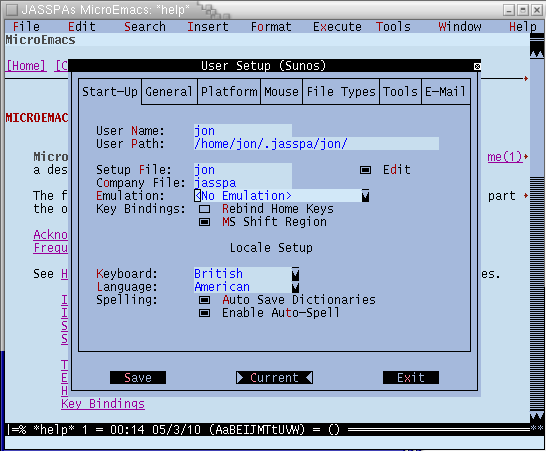
\includegraphics[keepaspectratio,height=3in]{usersetup}
    \caption{User Setup Dialog}
    \label{fig:usersetup}
  \end{center}
\end{figure}

    Navigation within the dialog is performed using the mouse and/or
    \texttt{TAB} and cursor keys. The \texttt{SPACE} key is used to open a
    drop down dialog. The configuration may be saved permanently using
    \textbf{Save} and installed into the current session using
    \textbf{Current}.

\subsubsection{Home/End Key Behavior}

    \textbf{User Setup::Start-Up::Rebind Home Keys}

    The behavior of the Home/End key is to move to the start/end of the
    buffer. When the option is enabled then the key behavior is changed to
    start/end of line.

\subsubsection{Microsoft Shift Region Control}

    \textbf{User Setup::Start-Up::MS Shift Region}

    Microsoft Shift Region Control when enabled emulates the Microsoft region
    selection behavior of the cursor keys when the \texttt{SHIFT} key is
    pressed. The cursor keys select a region whilst the \texttt{SHIFT} key is
    depressed.

\subsubsection{Nedit key bindings}

    \textbf{User Setup::Start-Up::Emulation} = \textbf{NEdit v5}

    \textbf{NEdit} key bindings are emulated when NEdit emulation is selected.

\subsubsection{GNU Emacs key bindings}

    \textbf{User Setup::Start-Up::Emulation} = \textbf{GNU Emacs}

\end{document}
